\documentclass[11pt]{article}

\usepackage[margin=1in]{geometry}
\usepackage{amsmath,amssymb,amsthm}
\usepackage{booktabs}
\usepackage{enumitem}
\usepackage{graphicx}
\usepackage{hyperref}
\hypersetup{colorlinks=true,linkcolor=blue,citecolor=blue,urlcolor=blue}

\newtheorem{proposition}{Proposition}
\newtheorem{remark}{Remark}
\DeclareMathOperator*{\argmax}{arg\,max}
\newcommand{\R}{\mathbb{R}}
\newcommand{\E}{\mathbb{E}}
\newcommand{\PR}{\mathbb{P}}
\newcommand{\MMD}{\mathrm{MMD}}
\newcommand{\Gcal}{\mathcal{G}}

\title{\textbf{Non-Uniqueness of Distribution-Shift Attribution,\\
and Why We Localize Subsets Instead}}
\author{Technical note}
\date{}

\begin{document}
\maketitle

\begin{abstract}
For a marketplace comparing an existing batch of data against a new batch, we
show a basic \emph{impossibility}: the \emph{total} distribution shift is
identifiable and order-invariant, but the \emph{per-feature contribution} to it
is not uniquely defined --- it depends on the order in which features are
considered. We demonstrate this empirically with random feature-addition paths
under two metrics: Maximum Mean Discrepancy (MMD) for covariate shift $P(X)$ and
the pseudo-outcome / $R$-risk for concept drift $P(Y\mid X)$. The consequence is
methodological: at any level of the entity hierarchy one should \emph{localize a
responsible subset} (well-posed) rather than attribute per-feature proportions
(ill-posed). We give the construction, the empirical result, the resulting
multi-level drill-down, a worked business example, and how such a system should
be evaluated.
\end{abstract}

\section{Setup}

Orders (observations) carry raw attributes and are labelled by batch
$W\in\{0,1\}$ (existing vs.\ new). We roll orders up to an entity axis
$\mathsf e$ (merchant, buyer, item, region, $\dots$) with a feature map $\Phi$
producing an entity--feature matrix $x\in\R^{p}$ (rich + rolling aggregations),
with features grouped by raw attribute, $g:\{1,\dots,p\}\to\Gcal$. Let $P_0,P_1$
be the two-batch feature distributions. A characteristic-kernel MMD measures
covariate shift, $\MMD^2(P_0,P_1)=0\iff P_0=P_1$; with batch as ``treatment'',
the $R$-risk of the induced pseudo-outcome regression measures concept drift and
is insensitive to pure covariate shift.

\section{Path-order attribution and its non-uniqueness}

Let $T(S)$ be a shift metric ($\MMD^2$ or $R$-risk) evaluated on the feature
subset $S\subseteq\{1,\dots,p\}$. Given an ordering $\pi$ of the features, the
\emph{addition path} is the curve $S_0=\emptyset\subset S_1\subset\dots\subset
S_p$ with $S_k=\{\pi_1,\dots,\pi_k\}$, and the marginal credited to feature
$\pi_k$ is $T(S_k)-T(S_{k-1})$. Sampling many random $\pi$ and averaging the
credits yields the Shapley value; but the credits along any single path are what
a ``how much did feature $f$ contribute'' question actually asks.

\begin{proposition}[Total identifiable, path non-unique]
The endpoint $T(S_p)=T(\{1,\dots,p\})$ is invariant to the order $\pi$: the total
shift is uniquely defined and estimable. The intermediate values $T(S_k)$,
$0<k<p$, and hence the per-feature marginals, are \emph{not} invariant to $\pi$
whenever the features are dependent; there is no order-free ``contribution of
feature $f$''. Shapley restores uniqueness only by \emph{averaging over all
orders}, i.e.\ by adopting a convention, not by identifying a truth.
\end{proposition}

\paragraph{Empirical demonstration.} We draw random feature-addition paths on the
repository's banded-Toeplitz covariate-shift and concept-drift DGMs and record
the metric at every step. Figure~\ref{fig:fan} shows the result: all paths
converge to the same full-set total (red, order-invariant), but the accrual
curves fan out in between; the shaded band is the \emph{irreducible attribution
ambiguity}. For concept drift the maximum gap between two orders is $\approx$ the
entire total ($\sim\!1.0$ against a total of $\sim\!1.06$): two feature orderings
can disagree about ``how much has been explained so far'' by essentially the
whole shift. The per-step standard deviation across orders is $30\!-\!40\%$ of
the total for both metrics.

\begin{figure}[t]
\centering
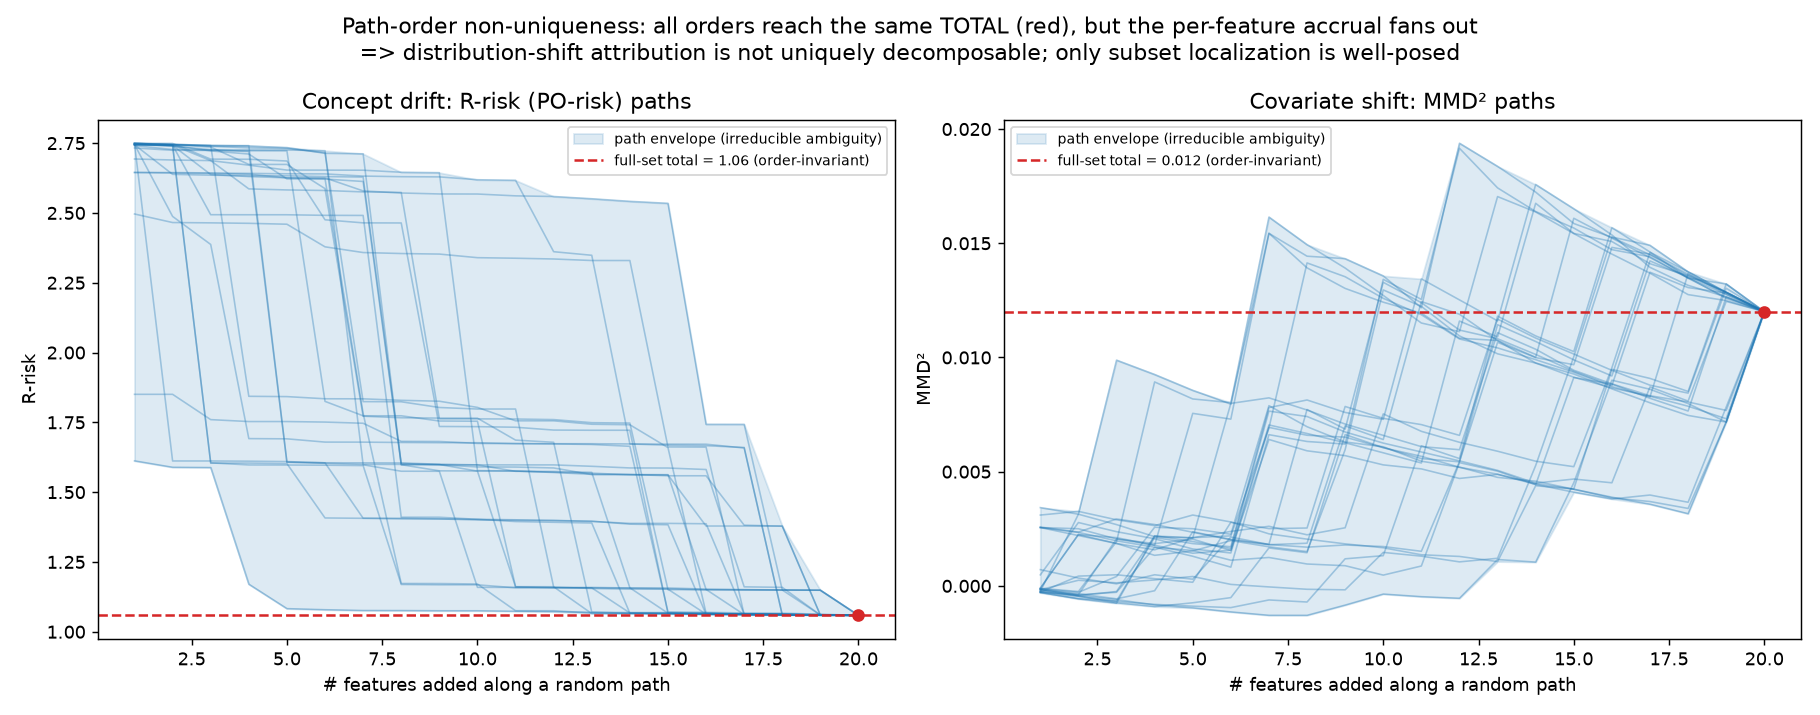
\includegraphics[width=\textwidth]{figures/path_nonuniqueness.png}
\caption{Random feature-addition paths. Every order reaches the same total
(red, order-invariant); the per-feature accrual fans out (shaded envelope $=$
irreducible ambiguity). Left: concept drift ($R$-risk); right: covariate shift
($\MMD^2$).}
\label{fig:fan}
\end{figure}

\begin{remark}[Any number of levels]
The argument is scale-free: it applies to features within one entity, and equally
to the coarser ``how much does each child level contribute'' question. Hence a
distribution shift is not uniquely decomposable at \emph{any} level of the
hierarchy.
\end{remark}

\section{The well-posed object: multi-level subset localization}

While ``how much'' is not identifiable, ``which subset carries the shift'' is: the
total is order-invariant, and the selection of the responsible group is stable
across attribution conventions and across resamples. We therefore localize
recursively, and never report proportions. The selection deliberately uses a
single global detection plus a leave-one-group-out ablation and a stability
check --- \emph{no multiple-testing machinery}, which keeps the procedure simple
and easy to trust:

\begin{enumerate}[leftmargin=2em]
\item \textbf{Detect} the shift globally with one MMD / $R$-risk permutation
test (order-invariant total).
\item \textbf{Localize (level 1)} to the responsible attribute-group subset by
\emph{leave-one-group-out (LOGO) ablation} --- the groups whose removal collapses
the shift --- kept only if stable across bootstrap resamples.
\item \textbf{Drill (level 2)} by \emph{restricting the order table to the
entities selected at level 1} (a conditional drill-down: keep only the flagged
subset's rows), then re-running the same selection on the next aggregation key
(e.g.\ item / product vertical) \emph{within that subset} --- again returning a
subset, not a share. Level 2 is therefore always evaluated on the level-1 subset,
not the whole population.
\item \textbf{Close the loop}: each selected subset carries an owner, a candidate
rule (a KS-optimal split threshold), a decision (monitor / reweight / retrain /
collect labels), and a trend status computed by diffing against the previous run.
\end{enumerate}

\section{Why LOGO, why these modalities, and why the subset is the unit}

\paragraph{Why LOGO.} We rank and select groups by the leave-one-group-out
ablation $\phi_g = T(\text{all}) - T(\text{all}\setminus g)$, the drop in the
shift metric when a group's features are removed. It is the right primitive here
for three reasons. (i) It answers the operational question directly --- ``if we
ignore or repair this group, does the detected shift disappear?'' --- which is
how an owner reasons and what makes the output actionable. (ii) It is a
\emph{conditional} importance (given all other features present), so a group is
credited only for what the rest does not already explain: it flags
\emph{non-redundant} drivers rather than everything merely correlated with the
shift. (iii) It is cheap ($K{+}1$ metric evaluations), its sign is meaningful
(removing a true driver lowers the metric; removing noise does not), and it needs
no attribution convention. Applied at the raw-attribute \emph{group} level it is
immune to the within-group correlation that would otherwise dilute every single
aggregation to near zero.

\paragraph{Why the subset --- not the feature --- is the effective unit.} By the
non-uniqueness result the total is order-invariant but the per-feature split is
not; the object that \emph{is} invariant and estimable is the contribution of a
whole subset (include or exclude the group as a unit). Empirically the
group-level answer is also stable across attribution conventions (standalone,
LOGO, and Shapley agree on \emph{which} groups) and across resamples, while the
per-feature answer is not. The grouping is not arbitrary: a real shift typically
enters through a raw signal --- a collection/definition change in GMV, a pricing
change, a new buyer cohort --- which moves \emph{all} of that signal's
aggregations together, so the raw-attribute group is the natural causal and
operational unit. Selecting that unit is therefore both statistically well-posed
(invariant, stable) and operationally meaningful (it maps to an owner, a rule,
and an action).

\paragraph{Why these modalities (MMD and PO-/R-risk).} A characteristic-kernel
MMD is zero iff the two batches share the same $P(X)$, and its LOGO drop is a
genuine reduction in a distributional distance that is sensitive to shifts in any
moment (mean, scale, tails), so it does not miss non-linear covariate shifts. The
PO-/R-risk targets the orthogonal, outcome-relevant question --- has $P(Y\mid X)$
changed --- and is insensitive to pure covariate shift, so the two modalities
cover the two failure modes without double-counting. Both are permutation-exact
and assumption-light, which is what makes a LOGO drop built on them a
trustworthy, convention-free number --- in contrast to Shapley, which becomes
unique only by averaging over an arbitrary set of orders.

\section{A worked business example}

\paragraph{Symptom.} In the new week's batch, the global test fires. Level-1
localization on the \emph{region} axis selects the activity subset --- concretely
the order-count feature \texttt{n\_orders} (and order-value aggregations) shifted
\emph{up} for a subset of users in region $R$: those buyers are placing more (and
larger) orders than the existing batch.

\paragraph{Non-uniqueness, honestly.} We do \emph{not} claim ``region $R$'s users
account for $43\%$ of the shift'' --- by the proposition that number is
order/convention dependent. We claim the shift is \emph{localized to} region
$R$'s user subset, with a stability of, say, $0.98$ and a split rule
$\texttt{n\_orders per user}>t$.

\paragraph{Drill one level --- \emph{inside} the flagged user subset.} We first
restrict the order table to exactly the level-1 subset (the flagged region-$R$
users, $\texttt{n\_orders per user}>t$), and only then aggregate those users'
orders on the \emph{item / product-vertical} axis and re-run the two-stage
selection. This conditional drill localizes the extra orders to a specific
\textbf{product vertical} (item category $C$) \emph{within that user subset}:
among the flagged region-$R$ users the surge concentrates in category $C$ (e.g.\
``fresh grocery''), not uniformly across the catalogue. The localization is thus
\textbf{product-vertical~$\times$~user-subset} (category $C$ conditioned on the
region-$R$ user segment), output as subset $=\{$region $R$ users, category $C\}$
with its own split rule and stability. Evaluating level 2 on the whole
population instead of on the level-1 subset would confound the two levels and is
explicitly avoided.

\paragraph{Action / closed loop.} The subset routes to the category-$C$ /
region-$R$ owner; the candidate rule becomes a monitor; the decision (e.g.\
\emph{reweight} if the mapping is unchanged, \emph{collect labels / retrain} if
the outcome relationship moved) is attached; the \texttt{trend} field marks it
\emph{resolved} once the subset stops flagging. The business learns \emph{where}
and \emph{who} and \emph{what to do} --- never a spurious percentage.

\begin{remark}[Why this is the right granularity]
``$43\%$ from category $C$'' would be unfalsifiable (non-identifiable) and
un-actionable. ``The new-batch order surge is localized to category $C$ among
region-$R$ users; here is the threshold and the owner'' is checkable, routable,
and monitorable --- it closes the loop.
\end{remark}

\paragraph{Results of the two-level procedure.} We inject a GMV covariate shift
concentrated in a \emph{single product item category} (Fresh Grocery) for new
merchants (200 merchants, 6 categories, 24k orders) and run the procedure.
Level 1 (merchant axis) selects the \texttt{gmv} attribute group by LOGO ablation
with full stability; the conditional Level 2 then drills into the
\textbf{product item category} and isolates \textbf{Fresh Grocery} exactly, while
every other category is non-significant (Table~\ref{tab:twolevel}). No
proportions are reported --- only the selected subsets, their ablation/gap
magnitude, stability, and permutation $p$.

\begin{table}[t]
\centering
\begin{tabular}{llrrr}
\toprule
Level (unit) & Candidate & LOGO / gap & Stability & Perm.\ $p$ \\
\midrule
\multicolumn{5}{l}{\emph{Level 1 --- merchant axis} \;(global $\MMD^2=0.281$, $p=0.003$)}\\
\;\; & \textbf{gmv} \;(selected) & $+0.283$ & $1.00$ & --- \\
\;\; & quantity & $-0.277$ & $0.85$ & --- \\
\midrule
\multicolumn{5}{l}{\emph{Level 2 --- product item category} \;(conditional on gmv, new vs.\ existing)}\\
\;\; & \textbf{Fresh Grocery} \;($c^\star$, selected) & $\mathbf{55.88}$ & --- & $\mathbf{0.002}$ \\
\;\; & Home \& Kitchen & $0.77$ & --- & $0.158$ \\
\;\; & Apparel & $0.58$ & --- & $0.240$ \\
\;\; & Electronics & $0.29$ & --- & $0.621$ \\
\;\; & Beauty & $0.26$ & --- & $0.583$ \\
\;\; & Toys & $0.03$ & --- & $0.932$ \\
\bottomrule
\end{tabular}
\caption{Two-level conditional subset localization (\texttt{fsds\_cross\_level.py}).
Level 1 selects the \texttt{gmv} attribute subset (LOGO ablation $+$ bootstrap
stability); the conditional Level 2 drills into the \textbf{product item
category} and selects exactly the shifted one, \textbf{Fresh Grocery}
(gap $=$ new$-$existing mean GMV within the category; merchant-block permutation
$p$). The order surge is localized to a single product item category, not spread
as proportions; ground truth is recovered at both levels.}
\label{tab:twolevel}
\end{table}

\section{How to evaluate such a system}

Because per-feature proportions are not identifiable, they must not be the yard
stick. Evaluate only identifiable targets:

\begin{center}
\begin{tabular}{lll}
\toprule
Target & Identifiable? & Metric \\
\midrule
Total / detection & yes (order-invariant) & test power; type-I under permuted labels \\
Subset localization & yes (convention-stable) & subset recall / precision vs.\ ground truth \\
Stability & yes & bootstrap selection frequency \\
Decision layer & yes (with labels) & downstream $\Delta$loss backtest \\
Per-feature proportion & \textbf{no} & --- (do not evaluate) \\
\bottomrule
\end{tabular}
\end{center}

The principle: judge a method by the questions it claims to answer (detection,
subset localization, stability, downstream impact), not by a question that is
provably unanswerable. The non-identifiability itself is demonstrated
empirically (Figure~\ref{fig:fan}), not hidden.

\section{Conclusion}

The total distribution shift is identifiable; its per-feature decomposition is
not. This is not a limitation of a particular estimator but a property of
dependent features under any additive path attribution. The productive response
is to \emph{localize responsible subsets} recursively down the entity hierarchy
and attach owner / rule / decision / trend to each --- turning an unanswerable
``how much'' into an operational ``which subset, who, and what to do''.

\end{document}
